
\documentclass[../ICIT-Paper-2024.tex]{subfiles}
% \documentclass[tikz,border=2mm]{standalone}
\usetikzlibrary{positioning}
\begin{document}

\paragraph{}
A Multilayer Perceptron (MLP) is a feedforward artificial neural network with fully connected neurons using a nonlinear activation function, typically organized in at least three layers, capable of distinguishing data that is not linearly separable. The MLP consists of three main layers: (1) the input layer, (2) one or more hidden layers, and (3) the output layer~\cite{8549859}. The process begins with the input layer receiving the raw data, which is then processed as it goes through the hidden layers. Each layer contains neurons that perform operations involving the weighted sum of their inputs, the application of an activation function (commonly ReLU), and the passing of the output to the next layer (see Figure~\ref{fig:neural_network}). The network’s prediction is usually computed in the output layer, providing the final result.


\begin{figure}
    \centering
    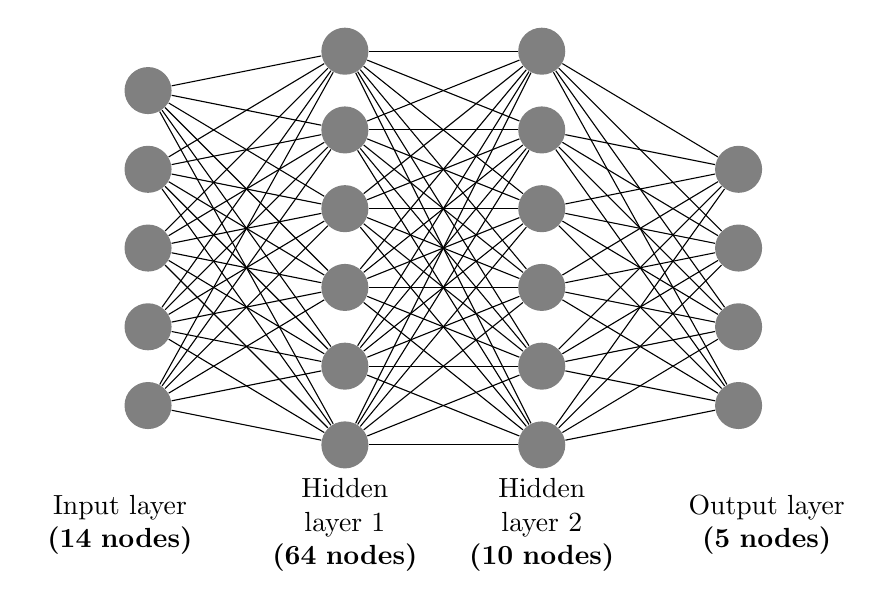
\begin{tikzpicture}[node distance=1.5cm]
        \tikzstyle{neuron}=[circle,fill=black!25,minimum size=17pt,inner sep=0pt]
        \tikzstyle{input neuron}=[neuron, fill=black!50];
        \tikzstyle{output neuron}=[neuron, fill=black!50];
        \tikzstyle{hidden neuron}=[neuron, fill=black!50];
        \tikzstyle{annot} = [text width=4em, text centered]
    
        % Input Layer
        \foreach \name / \y in {1,...,5}
            \node[input neuron] (I-\name) at (0,-\y) {};
    
        % Hidden Layer 1
        \foreach \name / \y in {1,...,6}
            \path[yshift=0.5cm]
                node[hidden neuron] (H1-\name) at (2.5,-\y) {};
    
        % Hidden Layer 2
        \foreach \name / \y in {1,...,6}
            \path[yshift=0.5cm]
                node[hidden neuron] (H2-\name) at (5,-\y) {};
    
        % Output Layer
        \foreach \name / \y in {1,...,4}
            \path[yshift=-1cm]
                node[output neuron] (O-\name) at (7.5,-\y) {};
        
        % Connect nodes
        \foreach \source in {1,...,5}
            \foreach \dest in {1,...,6}
                \path (I-\source) edge (H1-\dest);
    
        \foreach \source in {1,...,6}
            \foreach \dest in {1,...,6}
                \path (H1-\source) edge (H2-\dest);
    
        \foreach \source in {1,...,6}
            \foreach \dest in {1,...,4}
                \path (H2-\source) edge (O-\dest);
    
        % Annotate the layers
        \node[annot,below=1cm of H1-5, text width=6em] (hl1){Hidden layer 1 \\ \textbf{(64 nodes)}};
        \node[annot, below=1cm of H2-5, text width=6em](hl2) {Hidden layer 2 \\ \textbf{(10 nodes)}};
        \node[annot, left = 0.5 cm of hl1, text width=6em] {Input layer \\ \textbf{(14 nodes)}};
        \node[annot, right = 0.5 cm of hl2, text width=6em] {Output layer \\ \textbf{(5 nodes)}};
    
    \end{tikzpicture}
    \caption{Neural network architecture}
    \label{fig:neural_network}
\end{figure}



In the MLP application section, we customized the loss function to fit the problem of assigning 2 labels. With the input parameters, $\text{first\_y}$ representing the first label, $\text{second\_y}$ representing the second label, and $\text{y\_pred}$ representing the predicted value, the new loss function is defined as follows:


\begin{equation}
\text{SCC (Sparse Categorical Crossentropy)} = \sum_{c=1}^{C} \text{one\_hot}(y_{\text{true}}, c) \cdot \log(y_{\text{pred}}[c])
\end{equation}
\begin{equation}
\text{Loss} = -\frac{1}{N} \sum_{i=1}^{N} \min(\text{SCC}(\text{first\_y}[i], \text{y\_pred}[i]), \text{SCC}(\text{second\_y}[i], \text{y\_pred}[i]))
\end{equation}

\begin{itemize}
    \item $ N $: Number of samples.
    \item $ C $: Number of classes.
    \item $ \text{one\_hot}(y_{\text{true}}, c) $: One-hot encoding function transforms label $ y_{\text{true}} $ to a one-hot vector.
    \item $ y_{\text{pred}}[i, c] $: The predicted probability $ y_{\text{pred}} $ belongs to class $ c $.
\end{itemize}



\end{document}

